\subsection {Patched TIMELY}

\begin{figure}[t]
\center
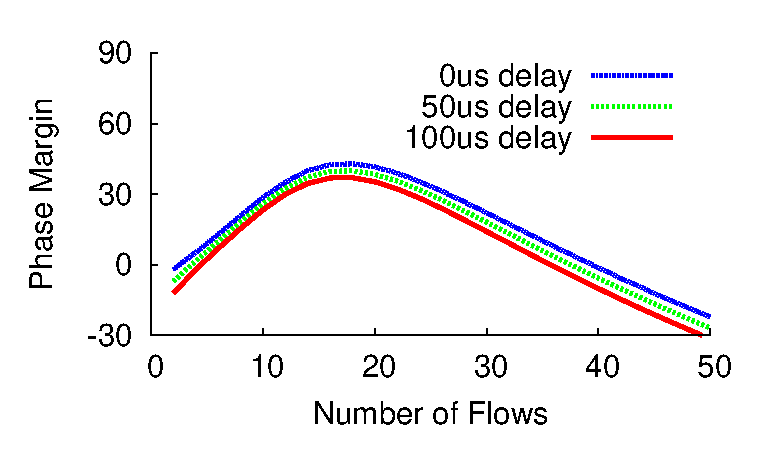
\includegraphics[width=0.33\textwidth]{figures/timely_stability.eps}
\caption{Patched TIMELY stability}
\label{fig:timely_stability}
\end{figure}


In order to ensure the protocol has a unique fixed point, and all flows get fair share and are stable at the fixed point,
we make two minor modifications over TIMELY.

First, we make the step of rate decrease rely on absolute queue length, instead of the gradient of queue length. 
This will ensure that there is only one fixed point for the queue length. In addition, all flow will have the same rate 
because the queue length, which is shared across flows, can uniquely determine the rate of each flow. This is 
similar to the use of ECN in DCQCN. The side effect is that, with different number of flows, the fixed point of 
queue will be different.

Second, we use a continuous weighting function $w(g)$ to make the transition between rate increase and rate decrease
smooth. This avoids the on-off behavior that causes oscillation, and stabilizes the protocol at the fixed point. 
This is similar to the fact that probabilistic ECN marking stabilizes TCP, QCN and DCQCN. With $w(g)$, we combine 
the two conditions of $g \le 0$ and $g>0$ in the $dR(t)/dt$ equation:


\begin{equation}
\small
\frac{{dR_i}}{{dt}} = \left\{ \begin{array}{ll}
\frac{\delta }{{\tau *}}, & q(t - \tau ') < C*{T_{low}}\\
\frac{{(1 - {w_i})\delta }}{{\tau *}} - \frac{{{w_i}\beta {R_i}(t)}}{{\tau *}}\frac{{q(t - \tau ') - q'}}{{q'}}, & Otherwise\\
 - \frac{\beta }{{\tau *}}(1 - \frac{{C*{T_{high}}}}{{q(t - \tau ')}})R_i(t), & q(t - \tau ') > C*{T_{high}}
\end{array} \right.\\
\label{eq:timely_fixed}
\end{equation}

where $w_i$, the weight of rate decreasing, is a function of $g_i$, and must satisfy $0 \le w_i(g_i) \le 1$ for any $g$. 
Intuitively, $w_i(g_i)$ is monotonically increasing with $g_i$, because larger RTT gradient should lead to larger 
weight of rate decreasing. In original TIMELY protocol, $w_i(g_i)$ is an indicator function of $g_i$, {\em i.e.,} 
$w_i(g_i)=1$ when $g \le 0$, and $w_i(g_i)=0$ when $g<0$. Here we simply use a linear function of $g_i$ for $w_i$:

\begin{equation}
\small
{w_i} = \left\{ \begin{array}{ll}
0, & {g_i \le  - \frac{1}{4}} \\
2{g_i} + \frac{1}{2}, & { - \frac{1}{4} < g_i < \frac{1}{4}} \\
1, & {g_i \ge \frac{1}{4}}
\end{array} \right.
\end{equation}

In Equation~\ref{eq:timely_fixed}, $q'$ is a reference queue length. We simply set it as $C*T_{low}$, 
so that we decrease the rate harsher if the queue length exceeds more than $C*T_{low}$. All the TIMELY
parameters remain the same except we set $\beta=0.008$ and $Seg=16KB$. 

\begin{thm}[Patched TIMELY's Unique fixed point.]
The system described in Equation~\ref{eq:timely_fixed} has a unique fixed point.
\end{thm}
\begin{proof}
Let the LHS of Equation~\ref{eq:timely_g} be 0, and $q(t - \tau ') - q(t - \tau ' - \tau *) = 0$ at the fixed 
point, we know $g_i^*=0$. Thus, $w_i^*=0.5$. Let the LHS of Equation~\ref{eq:timely_fixed} be 0. Because
all flows share the same queue length $q^*$, we have:

\begin{equation}
\small
R_1^* = R_2^* = ... = R_N^*
\end{equation}

The sum of all flow rates must be $C$ at the fixed point, therefore each flow has fair share $C/N$. 
\end{proof}

In addition, we can easily obtain the fixed point of queue length:
\begin{equation}
\small
{q^*} = \frac{{N{R_{AI}}q'}}{{\beta C}} + q'
\label{eq:timely_fixed_q}
\end{equation}

\begin{thm}[Patched TIMELY convergence.]
The system described in Equation~\ref{eq:timely_fixed} always converges to the unique fixed point.
\end{thm}

Here we provide a sketch of the proof. First, the queue length $q$ always
converges to the fixed point $q^*$. This can be proved by contradiction because whenever $q$ stabilizes
at $q>q^*$, we have ${\left. {\frac{{dR}}{{dt}}} \right|_{q > {q^*}}} < {\left. {\frac{{dR}}{{dt}}} \right|_{q = {q^*}}} = 0$, 
leading to queue length decrease. Vice versa holds for $q<q^*$. 

Second, once queue length converges to a stable state, we see $g_i$ converges to 0 by obtaining
the solution of the differential equation $\frac{{d{g_i}}}{{dt}} =  - \frac{\alpha }{{{\tau ^*}}}{g_i}$.

Finally, after $g_i$ converges to 0, which means $w_i=0.5$, we rewrite the $j$th flow's Equation~\ref{eq:timely_fixed} 
and subtract it from $i$th flow's. After simplification, we get:

\begin{equation}
\small
\frac{{d\left( {{R_i} - {R_j}} \right)}}{{dt}} = \frac{\delta }{{2Seg}}\left( {1 - \frac{N}{C}\left( {{R_i} + {R_j}} \right)} \right)\left( {{R_i} - {R_j}} \right)
\end{equation}

If one of flow ${i,j}$ is larger than the fair share $C/N$ while the other is smaller than $C/N$,
the rate different between them will decrease over time. Assuming ${{R_i} + {R_j}}$ does not change
much, we see that they converge exponentially over time by solving the differential equation.

We verify this using simulations. As shown in Figure TODO, flows with different initial rates converge 
to the fixed point and are stable without oscillation. 

\para{Stability.} We use the same technique as analyzing
DCQCN stability, {\em i.e.,} linearize the equations, Laplace transform and compute the phase margin 
of its characteristic equation. The phase margin result shows this system is stable when the number of 
flows is less than 40 (Figure~\ref{fig:timely_stability}). After 40 flows, the phase margin falls below 
0 rapidly because more flows lead to larger queue size (see Equation~\ref{eq:timely_fixed_q}), 
thus leading to larger feedback delay (see Equation~\ref{eq:timely_taup}). 
This leads to system instability. We conclude that with some minor tuning, TIMELY can be stable 
within a range of number of flows.